\chapter{Introduction}\label{ch:intr}
The phenomena of heavy-tailedness is widely observed in many
disciplines of science, for example, phase transition of matter and
black body radiation as studied in physics, neuronal avalanches in
biology, claim sizes of insurance mathematics and stock returns in
finance. The last application is indeed the focus of this thesis. To
discuss the phenomena in precise terms, we introduce the concept of
regular variation.

\section{Regular Variation}\label{sec:intro_regvar}
The concept of regular variation is defined by the following scaling
property: if a function $f$ on $(0, \infty)$ satisfies
\[
\lim_{x \to \infty} {f(c x) \over f(x)} = c^\alpha
\quad
\forall c > 0
\]
then we say $f$ is regularly varying with index $\alpha$.
$f$ can be written in the form $f(x) = {L(x) \over x^\alpha}$, where
$L(x)$ is a slowly varying function, i.e.
$\lim_{x \to \infty} {L(c x) \over L(x)} = 1$, $\forall c > 0$.
We call a random variable $X$ regularly varying with index
$\alpha \geq 0$ if it satisfies the tail balance condition in the
limit $x \to \infty$.
\[
\P(X > x) \sim p_+ {L(x) \over x^\alpha},\quad
\P(X < -x) \sim p_- {L(x) \over x^\alpha}, \quad
\text{for some } p_+, p_- > 0,\; p_+ + p_- = 1
\]

% Distribution functions, say $F(\cdot)$, whose survival function
% $\bar F(x) = 1 - F(x)$ satisfies the above scaling property, are
% observed in a variety of phenomena, 
When expanded to multiple dimensions, the scaling property of regular
variation is better described in terms of vague convergence to a
spectral measure $\mu_\alpha$: if a random vector $V$ satisfies
\[
{
  \P(X/|X| \in \cdot, |X| > c x)
  \over
  \P(|X| > x)
}
\overset{v}{\to} c^{-\alpha} \mu_\alpha(\cdot),
\quad
x \to \infty, \forall c > 0,
\]
then we say $X$ is regularly varying with index $\alpha$. Here
$\mu_\alpha$ is a probability measure on the unit sphere
\cite{buraczewski:damek:mikosch:2016}. It is called the spectral 
measure of $X$ and $\alpha$ is again the tail index.
If $X$ is regularly varying with index $\alpha$, then each component
and each linear combination of its components are regularly
varying with the same index $\alpha$. This follows from Feller
\cite{feller}, p. 278. Cf. also Jessen and Mikosch
\cite{JessenMikosch2006}, lemma 3.1, and Embrechts et. al.
\cite{embrechts:klueppelberg:mikosch:1997}, lemma 1.3.1.

Clearly, estimating the tail index $\alpha$ of a sequence
$X_1, X_2, \dots$ of regularly varying variables is particularly
important for understanding the behaviour of a heavy-tailed series. A
standard method proposed for this purpose is due to Hill
\cite{hill1975simple}:
\begin{equation}
  \label{eq:fhhty}
  \hat \alpha_H = \left[
    {1 \over k} \sum_{i=1}^k \log \left(
      X_{(i)} \over X_{(k+1)}
    \right)
  \right]^{-1},
\end{equation}
where $X_1, X_2, \dots, X_n$ is a sample whose tail index is the
subject of estimation, and $X_{(i)}$ is the $i$-th upper order
statistic of the sample. Several authors have contributed to showing
the weak consistency and asymptotic normality of the estimator
$\hat \alpha_H$, under the assumptions $k \to \infty, k/n \to 0$
as $n \to \infty$.

%% Mason \cite{mason:1982} first proved that the estimator
%% was consistent when $X_1, X_2, \dots$ were iid; later Rootz\'en,
%% Leadbetter and de Haan \cite{rootzen:leadbetter:dehaan1992} and Hsing
%% \cite{hsing:1991} proved its consistency when $X_1, X_2, \dots$ were
%% weakly dependent; and Resnick and St{\u a}ric{\u a}
%% \cite{resnick:starica:1995, resnick:starica:1997} proved its
%% consistency when $X_t$ was a linear process.

Figure \ref{fig:thjyuj} shows the Hill estimates of the tail indices
of daily stock return series from 3 sectors of the
{\em Standard \& Poor's 500} index \footnote{An American stock index
  comprising around 500 companies.}. The 2.5\% and 97.5\% quantiles of
the asymptotic normal distribution of the estimates are also
given. One can see the confidence bands are fairly large compared with
the estimated values. This certainly raises the question of how
similar they really are and if/how their variations can be explained by
economic arguments. We explore this topic in chapter
\ref{ch:TailParameters}.

\begin{figure}[htb!]
  \begin{minipage}{1.0\linewidth}
    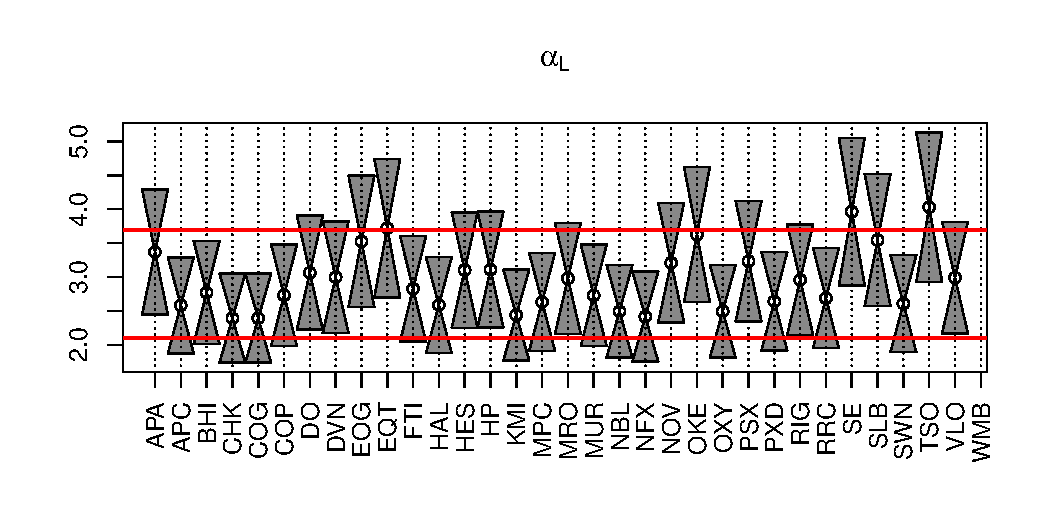
\includegraphics[width=\textwidth, trim={0, 0.8cm, 0, 2cm}, clip]
    {Energy_lower.pdf}
  \end{minipage}
  \begin{minipage}{1.0\linewidth}
    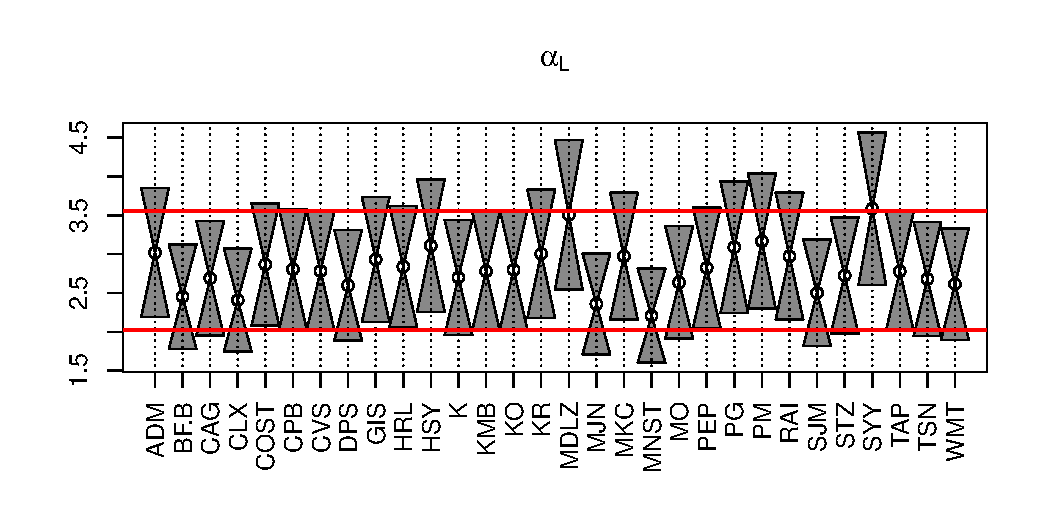
\includegraphics[width=\textwidth, trim={0, 0.8cm, 0, 2cm}, clip]
    {Consumer_Staples_lower.pdf}
  \end{minipage}
  \begin{minipage}{1.0\linewidth}
    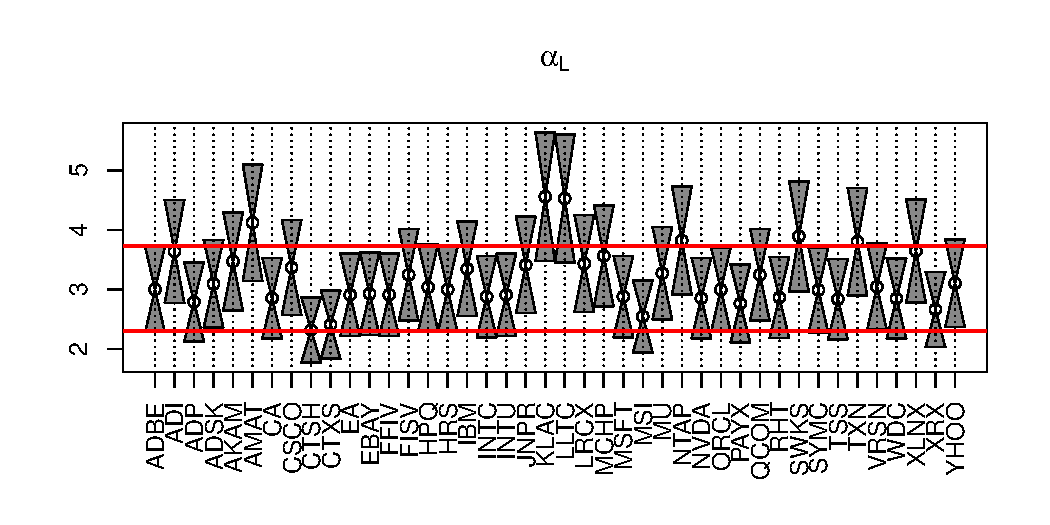
\includegraphics[width=\textwidth, trim={0, 0.8cm, 0, 2cm}, clip]
    {Information_Technology_lower.pdf}
  \end{minipage}
  \caption{\small Hill estimates $\hat \alpha_{50}$ of the lower
    tail-indices $\alpha$ of daily return series in sectors of the S\&P 500
    index. The data span from 1 January 2010 to 31 December 2014 and
    comprise $n=1304$ observations.
    The graphs from top to bottom correspond to the ``Energy'',
    ``Consumer Staples'' and ``Information Technology'' sectors.
    Each circle corresponds to a Hill estimate $\hat\alpha_{50}$; the gray
    triangles above and below it mark the 97.5\% and 2.5\% quantiles
    of its approximate normal distribution; see \eqref{eq:2} and the
    discussion following it for an interpretation.
    The lower and upper red lines mark the medians of the 2.5\% 
    and 97.5\% quantiles, respectively, evaluated from all stocks in
    the sector.
    The data are taken from {\it Yahoo Finance}; the labels on
    the horizontal axes are Yahoo symbols of the stocks. 
  }\label{fig:thjyuj}
\end{figure}

Random variables with regularly varying tails have some very nice
features: if $X_1$ and $X_2$ are both regularly varying with indices
$\alpha_1$ and $\alpha_2$, respectively, then $a_1 X_1 + a_2 X_2$ is
regularly varying with index $\min\{\alpha_1,
\alpha_2\}$ (cf. Mikosch and Jessen
\cite{JessenMikosch2006}). Moreover, if $X_1, X_2$ are iid,
$\P(a_1 X_1 + a_2 X_2 > u) \sim \P(a_1 X_1 > u) + \P(a_2 X_2 > u)$.

Now consider $p$ return series
$X_{i,t}$, $i=1,2,\dots, p; t=1,\dots,n$.
Suppose each of these series is a linear combination of $K$ factors
$Y_{j,t}$, $j=1,2,\dots,K$, the $j$-th of which is regularly varying
with index $\alpha_j$. Then by the summation property, each and every
$\{X_i\}$ is regularly varying with index $\min_{1 \leq j \leq K} \alpha_j$.
In practice a factor $Y_{i,t}$ is estimated as
$\hat Y_{j,t} = \sum_{i=1}^p a_{j, i} X_{i,t}$, where
$(a_{j, 1}, a_{j, 2}, \dots, a_{j, p})^\top$ is the $j$-th eigenvector
of the sample covariance matrix of
$\{X_{i,t}\}, i=1,\dots,p; t=1,\dots,n$, i.e. the eigenvector
associated with the $j$-th largest eigenvalue. 
For this reason, it is important to understand the eigensystem of the
sample covariance matrix of $\{X_{i,t}\}$. This topic is addressed in
chapters \ref{ch:bernoulli} and \ref{ch:extremes} of this thesis.

When a product of independent positive random variables, say $X_1
X_2$, involves one with regularly varying tails, a useful result is
that of Breiman \cite{breiman:1965}: assume $X_1$ is regularly varying
with index $\alpha$ and there exists $\epsilon > 0$ such that
$\E X_2^{\alpha + \epsilon} < \infty$.
Then $\P(X_1 X_2 > x) \sim \E X_2^{\alpha} \P(X_1 > x)$.
More generally, if $X_1, X_2$ are regularly varying with the same tail
index $\alpha$ or if $\P(X_2 > x) = o(\P(X_1 > x))$, then $X_1 X_2$ is
regularly varying with index $\alpha$.

In addition to Breiman's result, the following is also well-known,
assuming $X_1, X_2$ are positive independent random variables and
$X_1$ is regularly varying with index $\alpha$:
\begin{enumerate}
\item if $X_2$ is regularly varying with index $\alpha$ or
  $\lim_{x \to \infty} {P(X_2 > x) \over \P(X_1 > x)} = 0$, then $X_1
  X_2$ is regularly varying with index $\alpha$.
\item if $X_1, X_2$ are iid and $\E X_1^\alpha = \infty$, then
  ${\P(X_1 X_2 > x) \over \P(X_1 > x)} \to \infty$
\item if $X_1, X_2$ are iid and $\E X_1^\alpha < \infty$, then the
  only possible limit of ${\P(X_1 X_2 > x) \over \P(X_1 > x)}$ is
  $2 \E X_1^\alpha$.
\end{enumerate}
For an extensive summary of the regular variation properties of
functions of regularly varying random variables, see Mikosch and
Jessen \cite{JessenMikosch2006}.

% When considered as the multiplicative inverse of the parameter of the
% {\em Generalized Extreme Value} distribution, there are other methods
% in the literature for estimating the tail index, e.g. Pickand's 
% estimator \cite{pickands1975statistical} $\hat \alpha_P$ and the
% Deckers-Einmahl-de Haan estimator $\hat \alpha_{\text{DEH}}$
% \begin{eqnarray*}
% {1 \over \hat \alpha_P}
% &=&
% {1 \over \log 2}
% \log {
%   X_{(k)} - X_{(2k)}
%   \over
% X_{(2k)} - X_{(4k)}  
% } \\
% {1 \over \hat \alpha_{\text{DEH}}}
% &=&
% 1 + {1 \over \alpha_H} + {1 \over 2} \left(
%   {H \over \alpha_H^2} - 1
% \right)^{-1}
% \end{eqnarray*}
% where it is similarly assumed $k \to \infty$ and $k/n \to 0$ as $n \to
% \infty$. The Deckers-Einmahl-de Haan estimator makes use of Hill's
% estimator $\hat \alpha_H$ and computes
% \[
% H = \left[
%   {1 \over k} \sum_{i=1}^k \log \left(
%     { X_{(i)} \over X_{(k+1)} }
%   \right)^2
% \right]^{-1}
% \]
% Apparently $1/H$ can be interpreted as the 2nd empirical moment of
% $\log(X_{(i)}/X_{(k+1)})$ for $i \leq k$.
% A major drawback of Pickand's and Deckers-Einmahl-de Haan's estimators
% is that, when applied to estimating the tail index, they discard the
% information that the tail index is always positive, hence resulting in
% a larger confidence band compared with that obtained for Hill's
% estimator. Therefore we stick to Hill's estimator in the empirical
% work included in this thesis.

\section{Stochastic Recurrence Equation}
One of the most important dynamical mechanisms that lead to regularly
varying r.v. is stochastic recursion of the following form:
\begin{equation}
  \label{eq:rhjyu}
  X_t = A_t X_{t-1} + B_t, \quad t \in \mathbb Z
\end{equation}
where $X_t$ is a $d$-dimensional random vector, $A_t$ is a $d\times d$
random matrix and $B_t$ is a $d$-dimensional vector, random or
deterministic. The sequence $\{(A_t, B_t)\}_{t \in \mathbb Z}$ are
iid. The stationary solution to \eqref{eq:rhjyu} satisfies the fixed-point
equation $X \overset{d}{=} A X + B$, where $X$ and $(A, B)$ are
generic elements of the $\{X_t\}_{t \in \mathbb Z}$ and
$(A_t, B_t)_{t \in \mathbb Z}$ sequences.

Kesten \cite{kesten:1973} showed that, when $A_t$ are almost
surely non-negative, has no row or column of only zeros, and
$B_t$ is almost surely non-negative and is not equal to the null
vector with probability 1, then the solution $X$ to the equation
$X \overset{d}{=} A X + B$ is regularly varying with a positive index
$\alpha$, assuming the following conditions (M) and (A):
\begin{itemize}
\item Condition (M)
  \begin{enumerate}
  \item The top Lyapunov exponent
    \[
    \gamma = \inf_{n \geq 1} {1 \over n}\E \log \|A_n \cdots A_1\|
    \]
    is negative.
  \item There exists $\alpha > 0$ such that
    \[
    1 = \lambda(\alpha) = \lim_{n \to \infty} {1 \over n} \log \E \|A_n \cdots A_1\|^\alpha
    \]
  \item $\E (\|A_1\|^\alpha \log^+\|A_1\|) < \infty$
  \item $\E |B_1|^\alpha < \infty$
  \end{enumerate}
\item Condition (A) : The group generated by
  \[
  \{\log\rho(s): s = A_n \cdots A_1 \text{ for some } n \geq 1\}
  \]
  is dense in $\reals$, where $\rho(s)$ denotes the spectral
  radius of matrix $s$.
\end{itemize}
Upon these conditions, Kesten's theorem gives
\begin{equation}
  \label{eq:jorg}
  u^\alpha \P(u^{-1} V \in \cdot) \overset{v}{\to} \nu_\alpha(\cdot)
\end{equation}
where $\nu_\alpha$ is a non-null Radon measure on
$\reals^d_+ \setminus \{0\}$ with the property
$\nu_\alpha(a A) = a^{-\alpha} \nu_\alpha(A)$.

In addition to non-negative matrices, two other classes of random
matrices have been shown to lead to power-law tails via the recurrence
relation \eqref{eq:garchpq_sre}. Alsmeyer and Mentemeier
\cite{alsmeyer:mentemeier:2012} considered invertible matrices whose
distribution has a density. Let $M(d, \reals)$ denote the space of
$d \times d$ matrices with real entries that are invertible with
probability 1. They replaced Kesten's condition
$\E (\|A\|^\alpha \log^+\|A\|) < \infty$ with a stronger
counterpart
$\E [\|A\|^\alpha (\log^+\|A\| + \log \|A^{-1} \|)] < \infty$,
and lifted the condition (A). In addition, they assumed
\begin{enumerate}
  \item The Markov chain $X_n$ on $\sphere^{d-1}$, namely
    $X_n = A_n X_{n-1} / |A_n X_{n-1}|$, is irreducible, i.e. for any open
    set $U \subset \sphere^{d-1}$ and any $u \in \sphere^{d-1}$, 
    $\exists n \geq 1$ such that $\P(X_n u \in U) > 0$.
  \item There exist $N \geq 1$, $c, \epsilon > 0$ and an invertible
    matrix $\bar A \in M(d, \reals)$ such that for any set
    $C \subset M(d, \reals)$, it holds true
    $\P(A_N \cdots A_1 \in C) \geq c |B_\epsilon(\bar A) \cap C|$,
    where $|\cdot|$ denotes the Lebesgue measure.
\end{enumerate}
These assumptions are termed conditions (id). Furthermore, they assumed
that there was no point in $\reals^d$ such that the recurrence
equation \eqref{eq:garchpq_sre} was stuck at this point with probability 1: 
$\P(A X + B = X) < 1$ for all $X \in \reals^d$. With these
assumptions, they showed
\[
\lim_{u \to \infty} u^\alpha \P(\inn{x, V} > u) = e_\alpha(x)
\]
where $x \in \sphere^{d - 1}$ and $e_\alpha(\cdot)$ is a continuous
function on $\sphere^{d-1}$.

The second of the (id) conditions, which is satisfied when the
distribution of $A$ has a Lebesgue density, can actually be lifted if
stronger moment conditions are imposed on $A$ and $B$, and in
addition, a proximity condition is satisfied by the support of
$A$. This is the result of Guivarc'h and Le Page.
\cite{guivarc:page:2016}. Let $G_A$ denote the semi-group generated
by $\{\Pi_n: \Pi_n = A_n \cdots A_1, A_i \in M(d, \reals)\}$. The
authors assumed
\begin{enumerate}
  \item There is no finite union $W$ of proper subspaces of $\reals^d$
    that satisfies $\forall a \in G_A, a W = W$.
  \item $G_A$ contains a proximal element, i.e. an element $a$ whose
    largest singular value is an algebraically simple eigenvalue of $a$.
\end{enumerate}
These two assumptions are termed (ip) conditions. Replacing the (id)
conditions of Alsmeyer and Mentemeier with (ip) and the moment
conditions of the former with
\[
\E \|A\|^{\alpha + \delta} < \infty, \quad
\E (\|A\|^{\alpha} \|A^{-1}\|^{\delta}) < \infty, \quad
\E (|B|^{\alpha + \delta} < \infty),\quad
\text{ for some }\delta > 0
\]
Guivarc'h and Le Page proved the vague convergence result of \eqref{eq:jorg}.

Bollerslev \cite{bollerslev:1986} showed that the fixed-point equation
$Y \overset{d}{=} A Y + B$ has a unique, strictly stationary solution
$Y$ with finite variance if and only if
\begin{equation}
  \sum_{i=1}^p \alpha_i + \sum_{j=1}^q \beta_j < 1
  \label{eq:bollerslev:intro}
\end{equation}

\section{GARCH models}
Introduced by Bollerslev \cite{bollerslev:1986} in 1986,
{\em Generalized Autoregressive Conditional Heteroscedasticity}
(GARCH) models have been hugely popular for modelling volatility of
financial time series and have inspired numerous variants.
A GARCH($p, q$) model is a stationary process
$\{X_t\}_{t \in \mathbb Z}$satisfying
\begin{eqnarray*}
  X_t &=& \sigma_t Z_t \\
  \sigma_t^2 &=& \omega + \sum_{i=1}^p \alpha_i X_{t-i}^2 +
  \sum_{j=1}^q \beta_j \sigma_{t-j}^2
\end{eqnarray*}
where $\{X_t\}$ is a return series, e.g. stock returns, foreign exchange
rates, interest rates, etc; $\{Z_t\}$ is an iid, mean 0, unit-variance
sequence, $\sigma_t^2$ is the variance of the distribution of $X_t$
conditional on
$\{(X_i, \sigma_i^2)\}_{i=0}^{t-1}$; $\omega, \{\alpha_i\}_{i=1}^p,
\{\beta_i\}_{i=1}^q$
are non-negative parameters of the model. The GARCH($p,q$) recurrence
equation is of the form of \eqref{eq:rhjyu}. With appropriate
conditions, $\sigma_t^2$ is shown to be a positive Harris recurrent
Markov chain (cf. Bollerslev \cite{bollerslev:1986} and Buraczewski et al.
\cite{buraczewski:damek:mikosch:2016}), whose stationary distribution
has regularly varying tails. The tail index $\alpha$ is given by
\begin{equation}
  \label{eq:grgbg}
  \lim_{n \to \infty} {1 \over n}\log\E\|A_n \cdots A_1\|^\alpha = 0,
\end{equation}
where $\{A_i\}_{i \in \mathbb Z}$ are iid matrices whose entries are
functions of $\{\alpha_i\}_{i=1}^p$, $\{\beta_i\}_{i=1}^q$ and
$\{Z_t^2\}$:
\[
A_i =
\begin{pmatrix}
  \alpha_1 Z_{t-1}^2 + \beta_1 & \beta_2 & \cdots &
  \beta_{q-1} & \beta_q & \alpha_2 & \alpha_3 &
  \cdots & \alpha_{p-1} & \alpha_p\\
  1 & 0 & \cdots & 
  0 & 0 & 0 & 0 & \cdots & 0 & 0 \\
  \vdots & \vdots & \ddots & 
  \vdots & \vdots & \vdots & \vdots &
  \ddots & \vdots & \vdots \\
  0 & 0 & \cdots &
  0 & 0 & 0 & 0 & \cdots & 0 & 0 \\
  0 & 0 & \cdots &
  1 & 0 & 0 & 0 & \cdots & 0 & 0 \\
  Z_{t-1}^2 & 0 & \cdots &
  0 & 0 & 0 & 0 & \cdots & 0 & 0 \\
  0 & 0 & \cdots &
  0 & 0 & 1 & 0 & \cdots & 0 & 0 \\
  \vdots & \vdots & \ddots &
  \vdots & \vdots & \vdots & \vdots &
  \ddots & \vdots & \vdots \\
  0 & 0 & \cdots &
  0 & 0 & 0 & 0 & \cdots & 0 & 0 \\    
  0 & 0 & \cdots &
  0 & 0 & 0 & 0 & \cdots & 1 & 0 \\    
\end{pmatrix}
\]
While GARCH models have been very successful for modelling financial
time series, it does have its drawbacks. For example, the tail
index is very sensitive to the model parameters $\{\alpha_i\}_{i=1}^p$ and
$\{\beta_i\}_{i=1}^q$. In applications, these parameters need to be
estimated from a sample and are always uncertain to some extent. For
this reason, there can be a significant discrepancy between the tail
index obtained via \eqref{eq:grgbg} with the model parameters
substituted for their sample estimates and the Hill estimate
\eqref{eq:fhhty}.

There exist various extensions of the univariate GARCH
model to the multivariate case. The most notable one is perhaps the
{\em constant conditional correlation} (CCC) model of Bollerslev
\cite{bollerslev:1990} and Jeantheau \cite{jeantheau:1998}. In the
bivariate case, CCC is the model 
\beao\bfX_t=
\left(\barr{l}X_{1,t}\\
X_{2,t}\earr\right)= \left(\barr{ll}\sigma_{1,t}& 0\\
0&\sigma_{2,t}\earr\right)\,\left(\barr{l}Z_{1,t}\\Z_{2,t}\earr\right)=\Sigma_t\,\bfZ_t\,,\qquad
t\in\bbz\,.
\eeao
Thus both return components $X_{i,t}$ have the form of a univariate
stochastic volatility model $X_{i,t}=\sigma_{i,t}Z_{i,t}$ 
with non-negative volatility $\sigma_{i,t}$ and an iid bivariate noise
\seq\ $(\bfZ_t)$ with zero mean and unit variance components.
We also have the specification
\begin{small}
\beam\label{eq:8:mikosch}
\bfY_t=\left(\barr{l}\sigma^2_{1,t}  \\  
\sigma^2_{2,t}\earr
\right)
&=& \left(
\barr{l}\alpha_{01}  \\\alpha_{02}   \earr\right)
+\left(\barr{cc}\alpha_{11} & \alpha_{12}  \\
      \alpha_{21} & \alpha_{22}\earr \right)\, 
\left(\barr{l}X_{1,t-1}^2  \\X_{2,t-1}^2   \earr\right)
 + \left(\barr{cc}\beta_{11} & \beta_{12}  \\\beta_{21} & \beta_{22} \earr
 \right)\,\left(\barr{c}\sigma^2_{1,t-1}  \\\sigma^2_{2,t-1}\earr
  \right)\nonumber\\
&=& \left(
\barr{l}\alpha_{01}  \\\alpha_{02}
\earr\right)+\left(\barr{cc}\alpha_{11}Z_{1,t-1}^2+\beta_{11}&\alpha_{12}Z_{2,t-1}^2+
\beta_{12}\\
\alpha_{21}Z_{1,t-1}^2+\beta_{21}& \alpha_{22}Z_{2,t-1}^2+\beta_{22}
\earr\right)\,\left(\barr{l}\sigma_{1,t-1}^2\\\sigma_{2,t-1}^2\earr
\right)\,,
\eeam
for positive $\alpha_{0i}$ and suitable non-negative 
$\alpha_{ij},\beta_{ij}$, $i,j=1,2$.
Writing
\beao
\bfB_t= \left(
\barr{l}\alpha_{01}  \\\alpha_{02}   \earr\right)\quad\mbox{and}\quad
\bfA_t=\left(\barr{cc}\alpha_{11}Z_{1,t-1}^2+\beta_{11}&\alpha_{12}Z_{2,t-1}^2+
\beta_{12}\\
\alpha_{21}Z_{1,t-1}^2+\beta_{21}& \alpha_{22}Z_{2,t-1}^2+\beta_{22}
\earr\right)\,,
\eeao
\end{small}
we see that we are again in the framework of a stochastic recurrence
equation but this time for vector-valued $\bfB_t$ and matrix-valued
$\bfA_t$:
\beam\label{eq:jan6b:mikosch}
\bfY_t=\bfA_t\,\bfY_{t-1}+\bfB_t\,,\qquad t\in\bbz\,.
\eeam
Kesten \cite{kesten:1973} also provided the corresponding theory  
for stationarity and tails in this case. \sta\ \cite{starica:1999}
dealt with the corresponding problems for CCC-GARCH processes,
making use of the theory in Kesten \cite{kesten:1973},
Bougerol and Picard \cite{bougerol:picard:1992}
and its
specification to the tails of GARCH models 
in Basrak et al.~\cite{basrak:davis:mikosch:2002}. \sta\ \cite{starica:1999} assumed the 
Kesten conditions for the matrices $\bfA_t$. These conditions ensure
that the product matrices $\bfA_1\cdots\bfA_n$ have positive entries
for sufficiently large $n$. Then Kesten's theory implies that all
components of the vector $\bfX_t$ have power-law tails with the same
index $\alpha$ and also that the \fidi s of the process $(\bfX_t)$ are
\regvary\ with index $\alpha$.
\par
Various GARCH modifications are derived by considering linear
combinations of CCC-GARCH models. The property of multivariate
\regvar\ of multivariate GARCH ensures that, after linear
transformations,  the new process in all components has again
power-law tails with the same index as the original GARCH process; see
Basrak et al.~\cite{basrak:davis:mikosch:2002}.
Models which are constructed in this way are
the Orthogonal GARCH model of
Alexander and Chibumba \cite{alexander:chibumba:1996}, its
generalization GO-GARCH by van der Weide \cite{Weide2002},  the Full
Factor GARCH model of Vrontos et al. \cite{vrontos2003full} and the
Generalized Orthogonal Factor GARCH model of Lanne and Saikkonen
\cite{lanne2007modelling}. These models are characterized by their
treatment of each series as a linear combination of factors, and each
of the factors is modeled as a GARCH process; see Silvennoinen and
Ter\"asvirt\"a \cite{silventeras:2009}.
\par
Not all choices of $\alpha$- and $\beta$-parameters in the model
\eqref{eq:8:mikosch} allow for an application of the Kesten theory. For
example, assume that only the diagonal elements $\alpha_{ii}$ and
$\beta_{ii}$ are positive. Then $\bfA_t$ is diagonal and, hence, the
condition that $\bfA_1\cdots\bfA_n$ have positive entries for
sufficiently large $n$  cannot be satisfied. In the latter situation,
both $(X_{1,t})$ and $(X_{2,t})$ are univariate GARCH
processes. Assuming the  conditions of the univariate Kesten-Goldie
theorem for each component process, $(X_{1,t})$ and $(X_{2,t})$ have
power-law tails  with indices $\alpha_1$ and $\alpha_2$, respectively,
given by the solutions to the equations  $\E [(\alpha_{ii}
Z_{i,t}^2+\beta_{ii})^{\alpha_i/2}]=1$, $i=1,2$. In this model, one
can introduce dependence between the two component series $(X_{1,t})$
and $(X_{2,t})$ by assuming dependence between the noise variables
$Z_{1,t}$ and $Z_{2,t}$. Another situation when the Kesten theory fails 
appears when $\bfA_t$ is an upper or lower triangle matrix: then the
products  $\bfA_1\cdots\bfA_n$ are always of the same triangular
type. 
Similar remarks apply when one considers a CCC model in general
dimension. Of course, one may argue that the latter models 
are not natural: they are degenerate since they do not allow 
for a linear relationship between all squared volatilities on a given
day.

\section{Stochastic Volatility models}
With the availability of high-frequency data, a different approach
than that of GARCH has been popularized for modelling volatility of
financial time series and has led to greatly improved accuracy of
prediction. This is the approach of stochastic volatility models.

In the pioneering work of Clark \cite{clark:1973}, the author modelled
the logarithmic price $Y_t$ as a subordinated stochastic process:
$Y_t = V_{\tau_t}$, where $V_i$ is a normally distributed random
variable with mean 0, variance $\sigma^2 i$ and independent
increments. $\tau_t$ is a real-valued, non-negative, non-decreasing
sequence with $\tau_0 = 0$. It models a time change. As pointed out by
Shepard and Andersen \cite{Shephard:Andersen:2009}, the log-price
process $Y_t$ is serially uncorrelated although potentially dependent,
provided that $V_t$ and $\tau_t$ are independent.

Later authors, e.g. Back \cite{back:1991} chose to model the log-price
process as a semimartingale, with increments of the martingale
component modelled as a product process:
\begin{eqnarray}
  Y_t &=& Y_0 + A_t + M_t \nonumber \\
  M_t - M_{t-1} &=& X_t = \sigma_t Z_t
  \label{eq:rtght}
\end{eqnarray}
where $A_t$ is a finite variation process and $M_t$ is a martingale
and hence $Y_t$ is a semimartingale. $\sigma_t$ is non-negative and
$Z_t$ is an iid process with 0 mean and unit variance. A convenient
choice of $\sigma_t$ is
\begin{equation}
  \label{eq:rfht}
  \log\sigma_t = \sum_{l \in \mathbb Z} \psi_l \eta_{t-l}  
\end{equation}
where $-1 \leq \{\psi_l\}_{l \in \mathbb Z} \leq 1$
is a sequence of real numbers with at least one non-zero element,
$\{\eta_t\}_{t \in \mathbb Z}$ is a iid sequence of random
variables. By Kolmogorov's 3-series theorem, the infinite series above
converges if and only if $\sum_{l \in \mathbb Z} \psi_l^2 < \infty$.
In particular, if $\{\eta_i\}_{i \in \mathbb Z}$ is normally
distributed with 0 mean, $\{\sigma_t\}_{t \in \mathbb Z}$ is
stationary and its marginal distributions are log-normal.

If, however, the sequence $\{Z_t\}_{t \in \mathbb Z}$ or
$\{\sigma_t\}_{t \in \mathbb Z}$ is regularly varying with index
$\alpha$ and some additional conditions are satisfied, $X_t$ is also
regularly varying with the same index. Specifically, if $Z_t$ is
regularly varying and $\sigma_t$ has a lighter tail, the conclusion
follows from Breiman's lemma. See \S\ref{sec:case1} of Jan\ss en et
al. i.e. chapter \ref{ch:bernoulli} of this thesis for more details.

If, instead, $\sigma_t$ has a heavier tail than $Z_t$, then $X_{i,t}$
is regularly varying assuming the following conditions:
\begin{itemize}
\item $e^\eta$ is regularly varying with index $\alpha$, where $\eta$
  is a generic element of the iid sequence
  $\{\eta_t\}_{t \in \mathbb Z}$, and
  \begin{equation}
    \label{eq:dfhty}
    \E e^{\alpha \eta} = \infty, \quad\text{ or }
    {\P(\eta_1 + \eta_2 > x) \over \P(\eta_1 > x)} \to c \in (0, \infty)
  \end{equation}
    where $\eta, \eta_1$ and $\eta_2$ are generic elements of the
    iid sequence $\{\eta_t\}_{t \in \mathbb Z}$.
\end{itemize}
Note the only finite limit for
${\P(\eta_1 + \eta_2 > x) \over \P(\eta_1 > x)}$ is
$\E e^{\alpha \eta}$. Hence the two conditions of \eqref{eq:dfhty}
are mutually exclusive. In chapter \ref{ch:bernoulli} we will see that
these two conditions lead to rather different behavior for
eigenvalues of the sample covariance matrix of stochastic volatility
processes of the form \eqref{eq:rfht}.

There are a few advantages in using stochastic volatility models. For
one thing, they are among the simplest models allowing for conditional
heteroscedasticity (cf. Andersen et
al. \cite{andersen:davis:kreiss:mikosch:2009}); for another thing,
they greatly improve the accuracy of predicting future volatilities
by taking advantage of high frequency data. Specifically, for the
semimartingale $Y_t$ we have
\begin{equation}
  \label{eq:jieg}
  [Y_{\delta}]_t
  =
  \sum_{j=1}^{\floor{t/\delta}}
  (Y_{j \delta} - Y_{(j-1)\delta})^2
  \overset{P}{\to} [Y]_t,
  \quad
  \delta \to 0.
\end{equation}
The object $[Y_\delta]_t$ is called the realized quadratic variation
in time series literature.
The convergence in probability follows directly from the definition of
quadratic variation.
%% When $\E Z_t = 0$, $[Y]_t = [M]_t$ 
Furthermore, Jacod \cite{jacod:1994} and
Barndorff-Nielsen and Shephard \cite{barndorff:shephard:2002} proved a
central limit theorem:
\[
  {[Y_\delta]_t - [Y]_t \over \sqrt{2 \delta \int_0^t \sigma_s^2 ds}}
  \overset{d}{\to} N(0, 1),
  \quad \delta \to 0
\]
Moreover, the structure $X_t = M_{t} - M_{t-1} = \sigma_t Z_t$ gives
$[Y_\delta]_t \overset{P}{\to} \int_0^t \sigma_s^2 ds$. Meanwhile,
It\^o's formula gives, for semimartingale $Y_t$,
\begin{eqnarray}
  Y_t^2 &=& [Y]_t + 2 \int_0^t Y_s d Y_s \nonumber \\
  &=& [Y]_t + 2 \int_0^t Y_s dA_s + 2 \int_0^t Y_s dM_s \nonumber \\
  \E Y_t^2 &=& \E [Y]_t + 2 \E \left( \int_0^t Y_s dA_s \right) \nonumber\\
  &\approx& \E [Y]_t, \quad \text{when $t$ is small} \label{eq:hytre}
\end{eqnarray}
\eqref{eq:hytre} and \eqref{eq:jieg} shows $\E Y_t^2$, or in other
words, the forecast of future squared return can be obtained as
$\E [Y_\delta]_t$, i.e. the forecast of future realized quadratic
variation. Since past realized quadratic variations are observable,
forcast of future $[Y_\delta]_t$ can be obtained using e.g. an ARFIMA
model.

\section{Contribution of this thesis}\label{sec:contr}

In this section we summarize our results from the research papers.

\subsection{Tail parameters of equity return series}
We have established that, in the case of an equity return series with
two-sided, functionally independent Pareto tails, investor
preference functionals are monotone increasing/decreasing with the
tail index/scale parameters. Thus in a market dominated by such
equities, the investors would pursue the largest tail index in the
market, leading to a shared common tail index for all equities.

The empirical results presented in section \ref{sec:1} suggest this
may well be the case for the ``Consumer Staples'' sector of S\&P 500,
given the Hill estimates of tail indices shown in figure \ref{fig:1}
and the largely positive results of tests for equal tail indices shown
in figure \ref{fig:PairTest}.

On the other hand, we have also seen that, when the left and the right
tails have the same indices, investor preference over the equity has
more sophisticated variations in the parameters' space including the
tail parameters of the equity, the interest rate, the investor's risk
apetite as captured by his utility function, and his threshold of
disappointment.

We also acknowledge that our model of the market and the investor is a
simple one, not accoounting for the dependence between equities, nor
the categorization of investors and their interactions. These are
potential topics of future work.

\subsection{Importance sampling estimator of GARCH(p,q) rare event probability}
  We propose an efficient importance sampling estimator for the rare
  event probability $\P(|V| > u)$ where $V$ is a vector following the
  stationary distribution of a GARCH($p, q$) process. Recall
  $V_t = A_t V_{t-1} + B$ is the matrix recurrence equation of a
  GARCH($p, q$) process. We emanate the process $\{V_t\}$ from a set
  $\mathcal C = \{V: |V| \leq M\}$ for some predefined positive
  constant $M$, and then we introduce a dual change of measure for the
  originally iid matrices $\{A_t\}$: for
  $t < T_u = \min\{i > 0: |V_i| > u\}$, we exponentially tilt the
  distribution of $A_t | X_{t-1}$, where $X_0 = V_0$ and
  $X_t = \prod_{i=1}^t X_0/|\prod_{i=1}^t X_0|$, so that
  $|A_t X_{t-1}|^\xi$ is more likely to take on large values and hence
  $|V_t|$ is more likely to exceed $u$. Once the exeedance has
  happened, we change the
  distribution of $\{A_t\}$ back to the original and continue the
  process until $V_t$ returns to the set $\mathcal C$. Along each
  simulated path emenating from $\mathcal C$ and ending in
  $\mathcal C$ we compute $N_u = \sum_{i=1}^K \1{|V_i| > u}$, where
  $K = \min\{i > 0: |V_i| \leq M\}$.

  The pursuit estimate of $P(|V|>u)$ is then a weighted average of
  $N_u$ computed along each path. The weight depends on the path.

\subsection{Eigenvalues of the sample covariance matrix of a   
stochastic volatility model}
We consider a multivariate heavy-tailed stochastic volatility model
and analyze the large-sample behavior of its sample covariance
matrix. We study the limiting behavior of its entries in the
infinite-variance case and derive results for the ordered eigenvalues
and corresponding eigenvectors. Essentially, we consider two different
cases where the tail behavior either stems from the iid\ innovations
of the process or from its volatility sequence. In both cases, we make
use of a large deviations technique for regularly varying time series
to derive multivariate $\alpha$-stable limit distributions of the
sample covariance matrix. While we show that in the case of
heavy-tailed innovations the limiting behavior resembles that of
completely independent observations, we also derive that in the case
of a heavy-tailed volatility sequence the possible limiting behavior
is more diverse, i.e.\ allowing for dependencies in the limiting
distributions which are determined by the structure of the underlying
volatility sequence.

\subsection{Extreme value analysis for the sample autocovariance
  matrices of time series}
We  provide some  asymptotic theory for the largest eigenvalues of a
sample covariance matrix of a $p$-dimensional \ts\ where the dimension
$p=p_n$ converges to infinity when the sample size $n$ increases. 
We give a short overview of the literature on the topic both in the
light- and heavy-tailed cases when the data have finite (infinite)
fourth moment, respectively. Our main focus is on the heavy-tailed
case. In this case, one has a theory for the \pp\ of the normalized
eigenvalues of the sample covariance matrix in the iid case but also
when rows and columns of the data are linearly dependent. We provide
limit results for the weak \con\ of these \pp es to Poisson or cluster
Poisson processes. Based on this \con\ we can also derive the limit
laws of various \fct als of the ordered eigenvalues such as the 
joint \con\ of a finite number of the largest order statistics, the
joint limit law of the largest eigenvalue and the trace, limit laws
for successive ratios of ordered eigenvalues, etc. We also develop
some limit theory for the singular values of the sample autocovariance
matrices and their sums of squares. The theory is illustrated for
simulated data and for the components of the S\&P 500 stock index. 
